\documentclass[border=4pt]{standalone}
\usepackage{pgfplots}\pgfplotsset{compat=1.18}
\usepackage{newtxtext}
\begin{document}
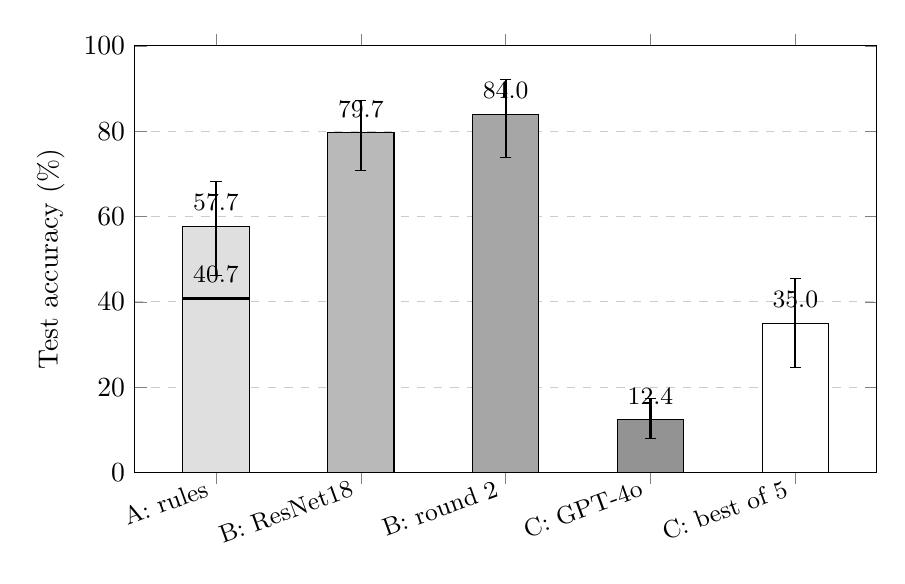
\begin{tikzpicture}
\begin{axis}[width=11cm,height=7cm,ybar,bar width=24pt,ymin=0,ymax=100,
 ylabel={Test accuracy (\%)},symbolic x coords={A,B1,B2,C,Cb},xtick={A,B1,B2,C,Cb},
 xticklabels={{A: rules},{B: ResNet18},{B: round 2},{C: GPT-4o},{C: best of 5}},
 xticklabel style={font=\small,rotate=20,anchor=east},enlarge x limits=0.14,ymajorgrids,grid style={dashed,gray!40},
 nodes near coords={\pgfmathprintnumber[fixed,precision=1,zerofill]{\pgfplotspointmeta}},every node near coord/.append style={font=\small,yshift=2pt},
 error bars/error bar style={black,thick}]
\addplot[fill=gray!25,draw=black,bar shift=0pt,error bars/.cd,y dir=both,y explicit] coordinates {(A,57.7) += (0,10.5) -= (0,11.5)};
\addplot[fill=gray!55,draw=black,bar shift=0pt,error bars/.cd,y dir=both,y explicit] coordinates {(B1,79.7) += (0,7.4) -= (0,8.9)};
\addplot[fill=gray!70,draw=black,bar shift=0pt,error bars/.cd,y dir=both,y explicit] coordinates {(B2,84.0) += (0,8.1) -= (0,10.1)};
\addplot[fill=gray!85,draw=black,bar shift=0pt,error bars/.cd,y dir=both,y explicit] coordinates {(C,12.4) += (0,5.0) -= (0,4.4)};
\addplot[fill=white,draw=black,bar shift=0pt,error bars/.cd,y dir=both,y explicit] coordinates {(Cb,35.0) += (0,10.5) -= (0,10.4)};
\addplot[only marks,mark=-,mark size=12pt,very thick,draw=black] coordinates {(A,40.7)};
\end{axis}
\end{tikzpicture}
\end{document}
